\documentclass[submit,techrep]{ipsj}
% \documentclass{ipsj}

\usepackage{graphicx}
\usepackage{latexsym}

\def\Underline{\setbox0\hbox\bgroup\let\\\endUnderline}
\def\endUnderline{\vphantom{y}\egroup\smash{\underline{\box0}}\\}
\def\|{\verb|}

\setcounter{巻数}{59}
\setcounter{号数}{1}
\setcounter{page}{1}

% \受付{2016}{3}{4}
% \再受付{2015}{7}{16}   %省略可能
% \再再受付{2015}{7}{20} %省略可能
% \再再受付{2015}{11}{20} %省略可能
% \採録{2016}{8}{1}

\begin{document}


\title{アプリ開発における異なる実践共同体の\\
可視化システムの開発}

\etitle{Development of visualization system of different community of practice in application development}

\paffiliate{Arcana}{株式会社スタジオ・アルカナ\\
Studio Arcana, Inc.}

\paffiliate{Meisei}{明星大学大学院情報学研究科情報学専攻\\
Department of Computer Science, Graduate School of Systems and Information Engineering, Meisei University}

\author{遠藤 勝也}{Katsuya Endoh}{Arcana}[k.endo@s-arcana.co.jp]
\author{武富 拓也}{Takuya Taketomi}{Meisei}
\author{尼岡 利崇}{Toshitaka Amaoka}{Meisei}

\begin{abstract}
本研究では,アプリケーション開発における異なる実践共同体の参加の過程を
可視化するシステムを開発した.
著者らは過去に質的アプローチの観点から実践共同体の概念を用いて,
異なる背景を持つプロジェクトメンバの関係のあり方が,
開発されるアプリケーションにどのような影響を及ぼすかという研究を行った.
その研究結果をもとにCSCW(Computer Supported Cooperative Work)の観点から,
アプリケーション開発の過程における,
背景の異なるプロジェクトメンバの関わり方を可視化するシステムの開発を行った.
本システムを使用することにより,
異なる背景を持つメンバが参加するアプリ開発チームにおいて,
アプリの設計から実装をメンバ間の関係構築のあり方そのものからデザインすることの
支援を目的としている.
\end{abstract}


\begin{jkeyword}
実戦共同体,CSCW,PBL,情報可視化
\end{jkeyword}

\begin{eabstract}
In this study, we have developed a system that visualizes the process of participation of different community of practice in application development.
In the past, the authors used the concept of Community of Practice (CoP) from the perspective of a qualitative approach, and how the relationships between project members with different backgrounds affect the applications being developed. I did a study. Based on the research results, we developed a system that visualizes the involvement of project members with different backgrounds in the process of application development from the viewpoint of CSCW (Computer Supported Cooperative Work). By using this system, the purpose is to support the design of the application from the way of building relationships between the members in the application development team in which members with different backgrounds participate.
\end{eabstract}

\begin{ekeyword}
Community of Practice, CSCW, PBL, Data Visualization
\end{ekeyword}

\maketitle

%1
\section{はじめに}

グローバル化のもとで社会は複雑化し,ICTの進歩はめざましく,
様々な業種や分野でソフトウェア・アプリケーション(以下,アプリと表記する)が
なくてはならないものとなっている.
現在のアプリの開発は,プログラマのみで完結することは少なく,
多様な背景を持つメンバと協働で行われる.
またアプリ開発において,様々なICTツールが導入され,
アプリの開発環境それ自体も変化している.


本研究は,過去に行った異なる背景を持つプロジェクトメンバの関係構築のあり方が,
開発されるアプリケーションのデザインにどのような影響を及ぼすかという
研究\cite{book1}の結果に基に行われたものである.
筆者らのこれまでの研究は大学の学部横断型PBL(Project based learning)を対象として行われており,
その結果をもとに本研究は,道具やテクノロジーの開発によって人々の協調的作業を
支援するシステムの開発を目標とした
CSCW(Computer Supported Cooperative Work)\cite{book2}の観点から
アプリケーション開発の過程における,
背景の異なるプロジェクトメンバの関わり方を実践共同体の概念から捉え,
可視化するシステムの開発を行う.


本システムを利用することで,
アプリを開発するプロジェクトメンバは,
開発されるアプリの機能やUser Interface(以下,UIと表記する)を,
技術や機能中心のみでタスクを決定するのではなく,
プロジェクトメンバが持つリソースを十分に利用できるような関係性からの観点も含めて
考えられるようになることを想定している.


%2
\section{アプリ開発におけるCSCWと実践共同体について}
\label{previous-research-cscw}

本章では,CSCWの背景とその発展に大きな影響を与えたサッチマンについて述べる.
また,次章で述べる著者らのこれまでの研究で分析した異なる専門性のメンバ同士の認識の違い
との関連から,サッチマンが抱えていた課題を取り上げる.
その課題に取り組むために有用であると思われる実践共同体の概念について考察を行う.


\subsection{CSCWとサッチマンの苦悩について}
CSCWの発展はエスノメソドロジーに依拠したL.サッチマンの影響を大きく受けている.
サッチマンは人々が社会生活を営むために用いる「やり方」を分析することを目的をする
エスノメソドロジー\cite{book3}の手法により,
人間の行動は状況依存的に組織されていることを主張した\cite{book4}.
このような社会の行為を状況との関わりの中で分析する研究は,
サッチマン以外にもE.ウェンガーが主張する実践共同体\cite{book5}の理論や,
日本においては上野直樹を中心とした状況論の研究が行われている\cite{book6}.

CSCWへの研究の発展に大きな貢献をしたサッチマンであったが,
同時に異分野横断的研究について,組織上の困難さを抱えていたと考えられる\cite{book7}.
その苦悩とは,異なる専門性にかかわる分業的な関係のあり方,
つまり,情報学研究とエスノメソドロジーの知識産出のプロセスや
前提とする認識論のズレも関係していたと考えられる\cite{book8}.
このような異なる背景を有するコミュニティのメンバ同士がコミュニケーションを行う場合,
異分野横断的研究に関わらず,
企業の部門間でも認識論の違いから主張の食い違いや対立が起きることもある\cite{book9}.

上記のような異なる専門性や背景をもつメンバ同士の関係について
どのように実践が行われているかの分析を行うには,
実践共同体の概念を用いることが有効であると考える.

\subsection{実践共同体と人工物との関わり}


実践共同体とは,成員の学習の促進あるいは知識を共有・創造といった
ある一定のテーマや目的のもとに構築された共同体である.
実践共同体は学習に関する認知科学やとくに教育工学と関わりが深い.
その理論は正統的周辺参加,ディスコース,布置といった概念を包括したものである.

実践共同体のイメージを図\ref{cop}に示す.
\begin{figure}[h]
  \centering
  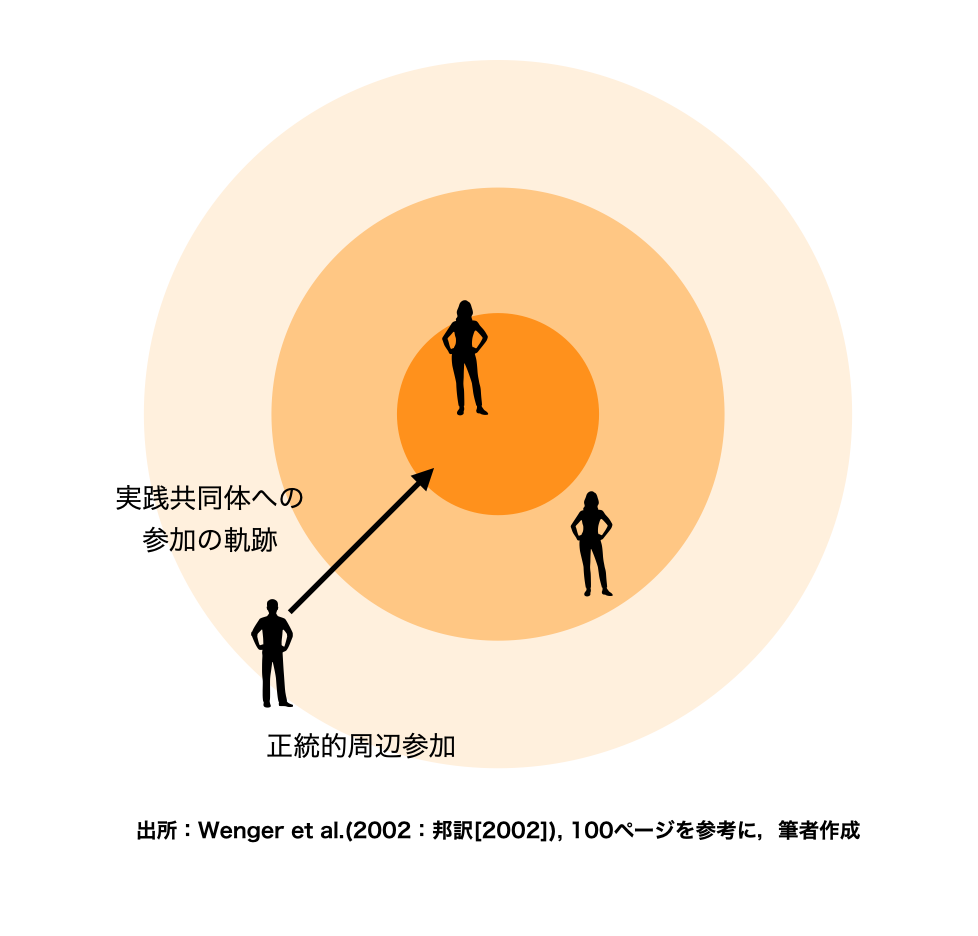
\includegraphics[width=0.5\textwidth]{img/cop.eps}
  \caption{実践共同体のイメージ図}
  \label{cop}
\end{figure}
正統的周辺参加とは,学習を成員がある実践共同体に加わり,
技能の獲得と成員のアイデンティティの発達を達成していくその動きとして捉える概念のことである.


加えて,正統的周辺参加として実践共同体に加わったその成員が,
その実践共同体内でどのような参加の過程を辿るかについては,
軌跡(Trajectory)という概念で表す.
ディスコースとは,実践共同体に共有される話し手のミクロな会話から
マクロな価値観まで含む文化のことを意味する\cite{book10}.
\begin{figure}[h]
  \centering
  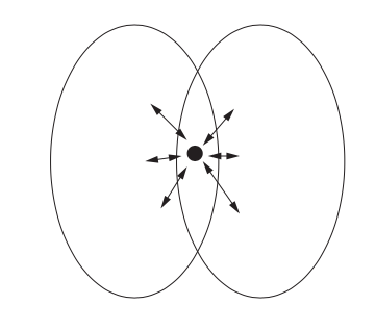
\includegraphics[width=0.5\textwidth]{img/overlap.eps}
  \caption{異なる実践共同体の協働のイメージ図}
  \label{overlap}
\end{figure}


布置とは,成員は単一の実践共同体のみに参加するものではなく,
複数の実践共同体に参加することを踏まえて,複数の実践共同体における
成員の振る舞いを捉える概念である\cite{book11}.
異なる実践共同体の重なりのイメージを図\ref{overlap}に示す.




実践共同体の概念は
学習という側面に関して多くの研究で効果が指摘されているが,
異なる実践共同体の関係構築のあり方と開発されるアプリへの影響についての
研究は著者が知る限りあまり行われていない.
しかし,上野\cite{book12}が示すように人工物は,
様々な組織間やコミュニティ間の調停,交渉の産物として形成されている.


そのため,人工物のデザインとはコミュニティのデザインであると述べているように,
実践共同体の概念を用いた分析は学習以外にも焦点を向ける有用性があると考えられる.
上記の理由から,実践共同体の概念を通して,
異なる背景を持つメンバ同士の関係のあり方が
アプリのデザインにどのよう影響しているかを分析する手法は有効であると考える.

%3
\section{アプリ開発におけるPBLの実践共同体の概念による分析}
\label{previous-research-pbl}

著者らのこれまでの研究は,情報学部情報学科(以下,情報学科と表記する)と
人文学部国際関係学科(以下,国際学科と表記する)が学部横断による
PBL型授業を対象に分析が行われた.
観察対象のPBL型授業のテーマは,「地域観光を促進するアプリの開発」である.
情報学科と国際学科を異なる実践共同体として捉え,
複数の実践共同体の関係構築のあり方が開発されアプリのUIに
どのように影響しているかについて,分析を行っている\cite{book13}.

国際学科と情報学科のそれぞれの実践共同体は,目的とする専門性や実践が異なる.
研究対象のPBL授業に参加する国際学科の学生は
英語でのプレゼンテーションが主な実践であり,
情報学科の学生はプログラミングやアプリ開発が主な実践となる.
 

PBL授業では,アプリの実装が完了した後で,
英語での成果発表という順番になるため,
異なる実践をもつ両学科の学生が
積極的にプロジェクトに参加する時期に齟齬がおきる傾向がみられた.


プロジェクトの前半はアプリ開発が主な作業となるため,
技術それ自体に価値を置く情報学科が積極的に参加し,
アプリ開発に携わった経験がほとんどない国際学科の学生は観察を主とした参加の態度になる.
これはアプリ開発という実践共同体に正統的周辺参加しているといえる.
他方,プロジェクト後半になると,アプリの成果発表があるため,
国際学科の学生がプロジェクトに積極的に参加し,
情報学科の学生が正統的周辺参加の態度を取る傾向が見られた.

それぞれ異なる実践共同体が築く関係のあり方として,
自分の専門性に関わるタスクしか関心を向けないという分業的な関係か
,または,自分の専門を超えて一緒に作業を行う時間を設ける協働的な
関係を築くかに分かれる.


分業的な関係のあり方でアプリ開発を進めた際,
タスクをこなす際に,部分最適化する傾向があり
制作された成果物は,異なる実践共同体の専門を組み合せるにとどまっていた.

他方,協働的な関係のあり方でアプリ開発を進めた際には,
短期的には非効率的に見えても,
アプリ開発の過程に
異なる実践共同体の実践,つまり,
プログラミング書いている最中の意味の交渉や目的の修正や共有が行われ,
お互いの専門性を融合して成果物を作成することを可能にした.
研究結果として,プロジェクトメンバの関係構築の在り方が分業的関係か協働的関係に応じて、
各プロジェクトメンバが所有する知識や技術といったリソースが
その人間関係のあり方に相応して開発プロセスに影響し、
アプリの機能やUIに現れるという示唆を得た.


本研究が開発したシステムは,アプリ開発支援システムとして,
異分野横断的なアプリ開発において,
異なる実践共同体が協働的な関係構築を行うことで,
お互いの実践を融合させてアプリ開発を支援することを目的としたシステムである.
使用場面として,ソフトウェアの開発手法の一つである
アジャイル開発に活用されることを想定している.
アジャイル開発とは機能単位の小さなサイクルで,
設計・開発・テストの工程を繰り返すことにより,
様々な状況の変化に対応しながら開発を進めていく手法である.
状況の変化に対応するため,
日毎にdaily scrumと呼ばれる短い時間での進捗の共有と反省を行う
打ち合わせの時間が設けられている.
開発したシステムはdaily scrumに活用されることが想定されており,
アプリ開発の要件から実装までを機能中心に組み立てるのではなく、
参加者それぞれの関心やスタンスを調整し
その関係のあり方そのものからデザインすることを可能にすることが期待されている.


 % アプリ開発支援ソフトウェアは,実践共同体の概念を参考に設計されている.
 % \begin{enumerate}
%     「正統的周辺参加」をTrelloの カードの移動,プロジェクトのタスクがどの共同体に属しいてるかをTrelloのラベル機能を用 いて表す.
% \end{enumerate}

\section{実践共同体の可視化システムについて}
\label{system-map}

図\ref{cop}と図\ref{overlap}で示したように,
従来までの実践共同体と参加者の関係性は,
ベン図の様な形で表されてきた.
% 従来の表現の欠点と本研究の可視化手法の強み
しかし,xxxやxxxの観点から,
xxxを表現するには適していないと考えられる.
そこで,本研究では,
プロジェクトメンバをノード,
プロジェクトメンバが協働でタスクを行った履歴をエッジとした,
ネットワーク構造として捉えることで,
xxxを可能にした.
本システムによって可視化したプロジェクトメンバの関係性を,
図\ref{cop-map-graph}に示す.

\begin{figure}[h]
  \centering
  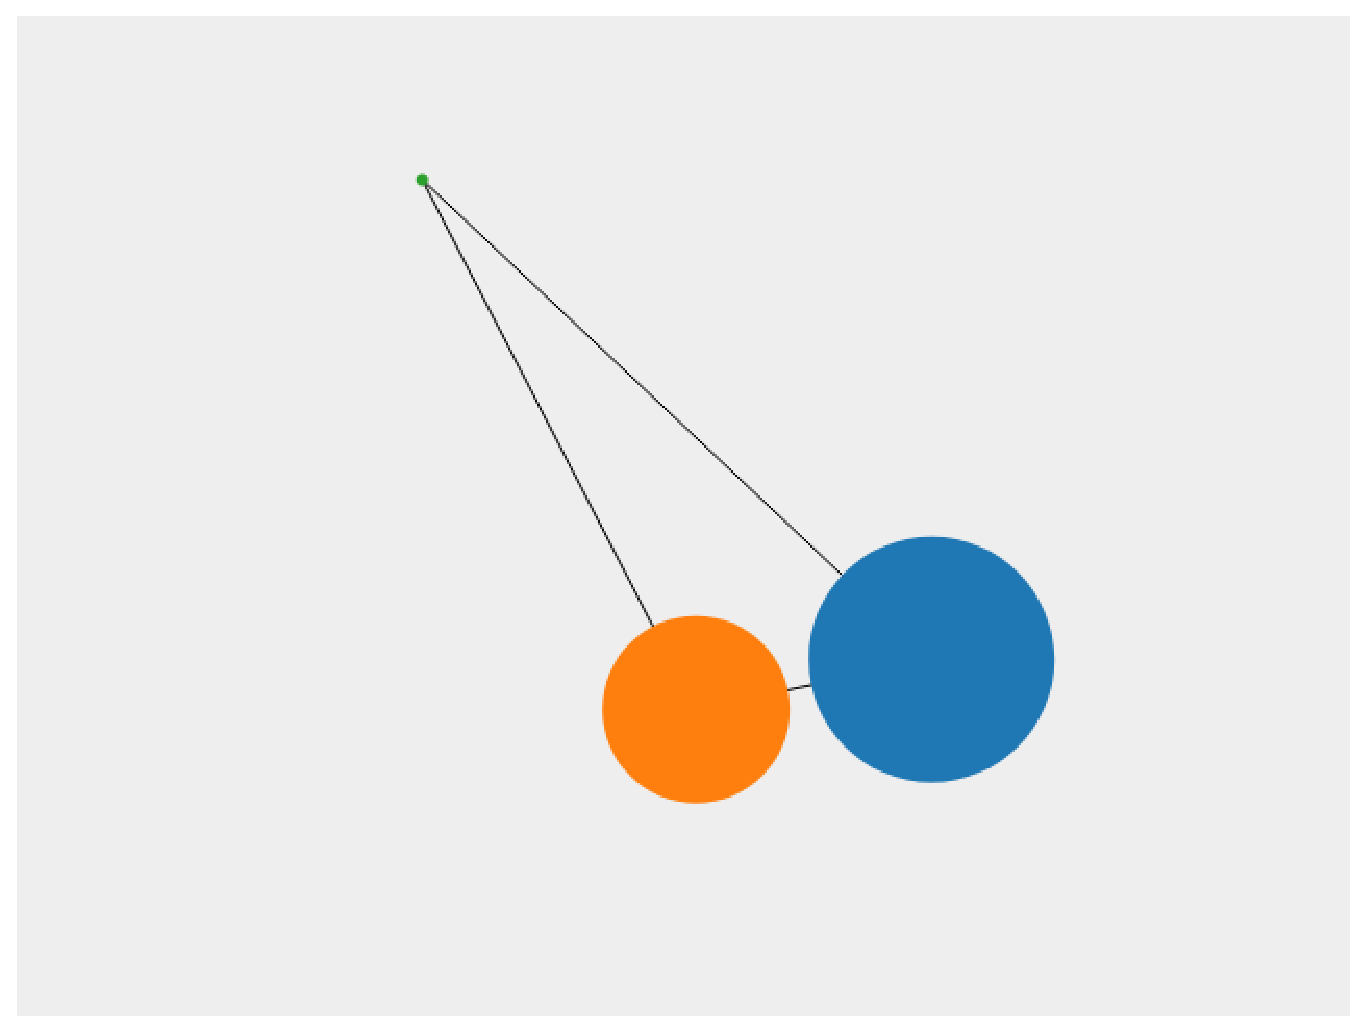
\includegraphics[width=0.5\textwidth]{img/cop-map-graph.eps}
  \caption{本システムによってプロジェクトメンバーの関係性を可視化した様子}
  \label{cop-map-graph}
\end{figure}

本システムは,
Atlassian社が提供するタスク管理ツールTrello\cite{trello}と連携して動作する.
Trelloによって管理しているタスクの情報を,
Web APIを使って取得することで,
分業的あるいは協働的にタスクをこなしているかを確認しながら,
アプリ開発を行うことが可能である.

本システムでは,ネットワーク構造のレイアウト手法として,力学モデルを採用している.
その際に,協働でタスクを行った回数によってエッジの強度を変化させている.
よって,多くのタスクを協働で行うほど,
ノード間の距離は近くなるように配置される.
% 共同ノード間の距離
% これにより,

また,プロジェクトメンバの所属先によってノードの色を変化させることで,
異なる実践共同体に所属するプロジェクトメンバが,
協働でタスクを行っている様子を観察することを可能にしている.
これにより,異なる色のノードがエッジでつながっている様子から,
布置を観察することを可能にしている.
本システムによって観察される布置の例を,
図 \ref{cop-map-overlap}に示す.

\begin{figure}[h]
  \centering
  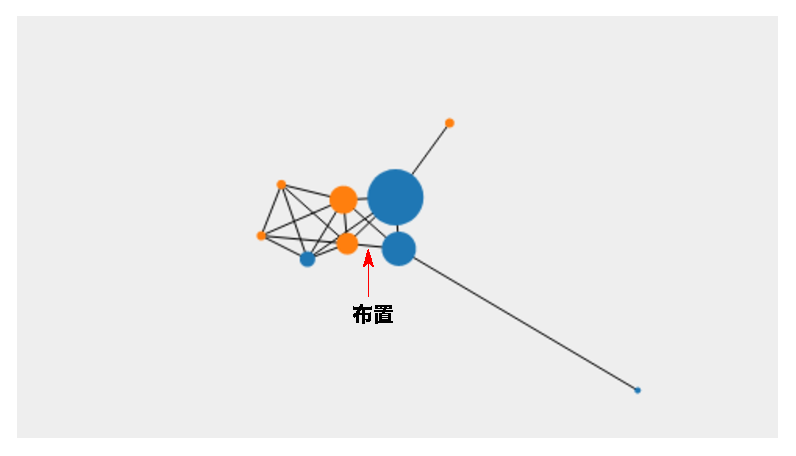
\includegraphics[width=0.5\textwidth]{img/cop-map-overlap.eps}
  \caption{本システムによって可視化された布置}
  \label{cop-map-overlap}
\end{figure}

さらに,タスクを行った回数の合計値によってノードの大きさを変化させている.
これにより,プロジェクトメンバが正統的周辺参加である可能性を観察することが可能である.
その一例として,ノードは小さいが,他のノードとの繋がりが見られる場合が挙げられる.
この場合は,観察対象となるプロジェクトメンバは,
タスクを行った回数は少ないが,
リソースへのアクセスが可能な状態だと考える事ができる.
本システムによって,
観察される正統的周辺参加である可能性のあるプロジェクトメンバーを図\ref{cop-map-lpp}に示す.

\begin{figure}[h]
  \centering
  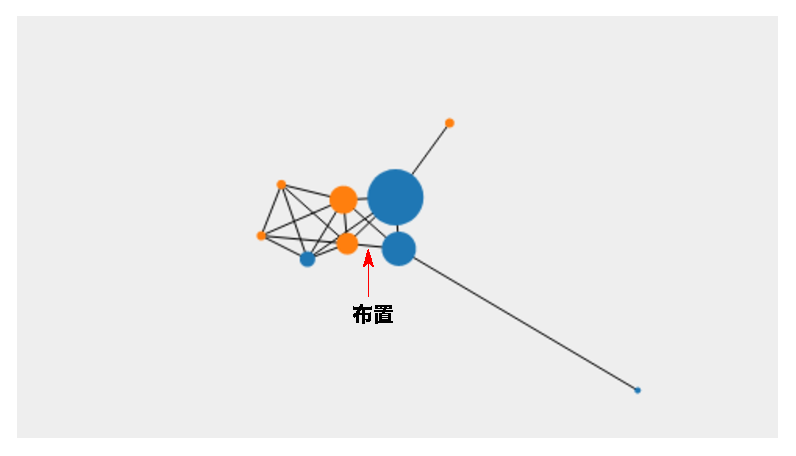
\includegraphics[width=0.5\textwidth]{img/cop-map-lpp.eps}
  \caption{本システムによって観察される正統的周辺参加である可能性のあるプロジェクトメンバー}
  \label{cop-map-lpp}
\end{figure}

以上のネットワーク構造を,プロジェクトの時系列順に変化させることで,
プロジェクトメンバの関係性の変化を観察することを可能にしている.
これにより,ノードの軌跡から,
進行状況によって変化していく,
プロジェクトメンバの軌跡を観察することを可能にしている.

また,本システムではインタラクティブにデータを観察することが可能である.
本システムで可能なインタラクションは,
ノードのドラッグアンドドロップと,ノードへのマウスオーバーである.
ノードをドラッグアンドドロップすることによって,
ネットワークのレイアウトを調整することが可能である.
また,メンバの詳細情報を確認する際には,
ノードにマウスオーバーすることで,
そのノードに対応するユーザ名を確認することが可能である.
これらのインタラクションにより,
より詳細にプロジェクトメンバの関係性を観察することが可能である.

% \begin{enumerate}
%    \item CoP
%    \item 布置
%    \item トラジェクトリー
%    \item 正統的周辺参加
% \end{enumerate}

% 本システムは,アプリケーションサーバとデータベース,
% 外部サービスであるTrelloから構成されている.
%
% タスクの履歴を,TrelloのWeb APIから取得して,
% 時系列順にネットワーク構造に整形することで可視化している.

%4
\section{今後の展望}

本研究で開発したシステムは,2021年度9月より実施される学部横断型PBLのアプリ開発を
行う際に使用される予定である.開発したシステムから,
メンバの背景と行為やメンバ間の交渉に着目し,
アプリの機能やUIがどのように決定されていくか 分析する予定である.
加えてアプリ開発支援ソフトウェアがアプリ開発の過程にどのように影響を及ぼすかまで含めて分析を行う.

% 遠藤が実装したい内容ついての記述

%5
\section{おわりに}

% 今後の展望と終わりにまとめてしまってもよい?

\begin{thebibliography}{9}


  \bibitem{book1}
  武富 拓也: {\it 複数の実践共同体の関係構築のあり方と観光アプリケーション開発への影響の考察},
    日本認知科学学会,
    (2016).
  \bibitem{book2}
  秋谷直矩:
  『組織コミュニケーションのデザイン』.:『ワークプレイス・スタディーズ はたらくことのエスノメソドロジー』 pp. 92-100,
  ハーベスト社(2017).

  \bibitem{book3}
  水川喜文・秋谷直矩・五十嵐素子:
  『ワークプレイス・スタディーズ はたらくことのエスノメソドロジー』 pp. 1-20,
  ハーベスト社(2017).

  \bibitem{book4}
ルーシー A. サッチマン, 佐伯胖・上野直樹・水川喜文・鈴木英幸訳:
『プランと状況的行為ー人間-機械コミュニケーションの可能性』,
産業図書(1999).

\bibitem{book5}
Wenger, E.: {\it Communities of practice : learning,
meaning, and identity.},
Cambridge :Cambridge University
Press. pp. 55-57 (1998).

\bibitem{book6}
上野直樹:
シリーズ人間の発達9 仕事の中での学習 状況論的アプローチ,
東京大学出版会(1999).

\bibitem{book7}
Suchman, L.,: {\it Working Relations of Technology Production and Use.},
Computer Supported Cooperative Work, :Springer,
2(1-2): 21-39 (1993).

\bibitem{book8}
  秋谷直矩:
  『メディアとデザインのインターフェース』.:『ワークプレイス・スタディーズ はたらくことのエスノメソドロジー』 pp. 227-236,
  ハーベスト社(2017).

\bibitem{book9}
  徐恩之: {\it 職能横断的なコミュニケーション
  におけるコンフリクトのトランスファー},
  組織科学,
  Vol. 45, No. 3 , pp. 22-34. (2012).

\bibitem{book10}
  ソーヤーりえこ:
  『社会的実践としての学習ー 状況的学習論概観』.『文化と状況的学習 実践,言語,人工物へ のアクセスのデザイン』 pp. 41-89,
  凡人社(2010).

\bibitem{book11}
  松本雄一: {\it 実践共同体概念についての一考 察: E. Wengerの実践共同体論を読み解く},
  関西学 院大学『商学論究』,
  Vol.64, No.3, pp. 347-409. (2017).

\bibitem{book12}
上野直樹:
『ネットワークとしての状況論』.『文化と状況的学習 実践,言語,人工物へ のアクセスのデザイン』 pp. 3-40,
凡人社(2010).

\bibitem{trello}
Atlassian.
"Trello"
\urlj{https://trello.com/ja}%
\refdatej{2021-07-25}.


\end{thebibliography}

\begin{biography}
\profile{n}{遠藤 勝也}{1992年生.2016年明星大学情報学部情報学科卒業.
2018年株式会社スタジオ・アルカナ入社.ウェブサービス開発に従事.芸術科学会会員.}
%
\profile{n}{武富 拓也}{1990年生.2016年明星大学人文部国際コミュニケーション学科卒業.
2019年明星大学情報学部実習指導員として勤務, 明星大学大学院情報学研究科情報学専攻博士前期課程(研究生). 社会言語科学会会員}
%
\profile{n}{尼岡 利崇}{1950年生.1974年架空大学大学院修士課程修了.
1987年同博士課程修了.工学博士.1977年架空大学助手.1992年情報処理大学助
教授.1987年同大教授.2000年から情報処理学会顧問.オンライン出版の研究
に従事.2010年情報処理記念賞受賞.情報処理学会理事.電子情報通信学会,
IEEE,IEEE-CS,ACM 各会員.}
\end{biography}

\end{document}
